\newpage
\section{White Rabbit PTP Core}

The WR PTP (Precision Time Protocol) Core (WRPC) \cite{WR-core:wiki} \cite{WR-core:manual} \cite{WRPC:ohwr}, figure \ref{fig:WRPC}, is an Ethernet MAC implementation capable of providing precise timing. 
It can be used for sending and receiving regular Ethernet frames between user-defined HDL modules and a physical medium. 
It also implements the White Rabbit protocol to provide sub-nanosecond time synchronization.

\vspace{5 mm}

\noindent The White Rabbit PTP Core can operate in one of the following modes:
 
\begin{itemize}
\item GrandMaster:
    \begin{itemize}
    \item[>] WR Master synchronized to an external 1-PPS and 10 MHz clock signal, propagates precise timing to other WR-compliant devices.
    \end{itemize}
\item Master:
    \begin{itemize}
    \item[>] WR Master with free-running oscillator, propagates precise timing to other WR-compliant devices.
    \end{itemize}
\item Slave:
    \begin{itemize}
    \item[>] synchronizes its internal oscillator to another WR Master device.
    \end{itemize}
\end{itemize}

\begin{figure}[H]
    \centering
    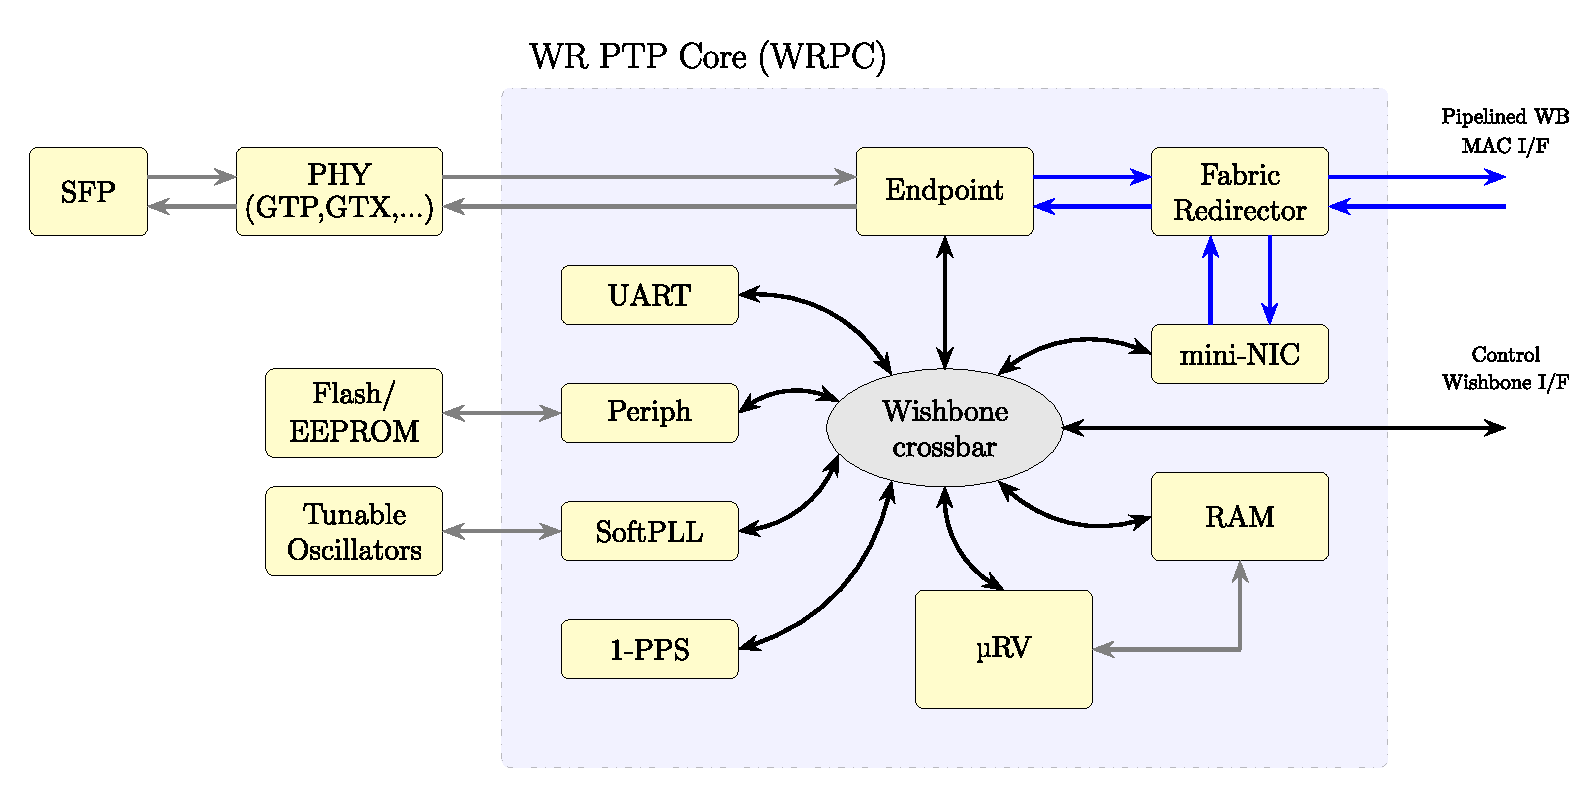
\includegraphics[width=15cm]{figures/WRPC.pdf}
    \caption{WR PTP (Precision Time Protocol) Core (WRPC).}
    \label{fig:WRPC}
\end{figure}

\noindent You can find the HDL description of the WRPC internal components in \cite{WRPC:modules}.

\subsection{\textmu RV}

The \textmu RV \cite{urv-core:ohwr} \cite{urv-core:wiki} \cite{Włostowski:2213516} (Micro RISC-V) core is a small-sized implementation of a 32-bit RISC-V core, targeted specifically at FPGAs developed by CERN. 

\begin{figure}[H]
    \centering
    
\includegraphics[width=5cm]{figures/urv_logo.png}
    \caption{\textmu RV logo.}
    \label{fig:urv}
\end{figure}

\begin{itemize}
\item Features:
    \begin{itemize}
    \item[>] Supports RV32IM instruction set. 
Division and multiply high instructions are optional and can be emulated to lower the FPGA footprint.
    \item[>] Target: FPGAs.
    \item[>] 4-stage pipeline (FDXW).
    \item[>] All instructions except taken branches/division in one clock cycle.
    \item[>] Code execution from internal memory block.
    \item[>] Wishbone bus (version B.4) for peripheral access.
    \item[>] Simple interrupt handling.
    \item[>] Verilog RTL code.
    \end{itemize}
\end{itemize}

\noindent Since \textmu RV is described in verilog and most of the WRPC component is in VHDL, it will be necessary to use a \textbf{mixed simulator} supported by VUnit.
In this context, one of the best options is \say{QuestaSim}.

\vspace{5mm}

\noindent \href{https://github.com/umarcor}{Umarcor} is planning to develop a container, hosted on our server, for this purpose. 
(DONE - Questa container, with and without VUnit, available on the lab server.)

\vspace{5mm}

\noindent \textbf{Task:} Learn how to generate a testbench using both HDLs: VHDL and Verilog.
(Initial mixed simulation test DONE - Unfortunately questa is a proprietary software and our server image cannot be distributed, so this example cannot be shown on GitHub, it is only available in our private GitLab repository.)
